\documentclass{article}

\usepackage{graphicx}
\usepackage{tikz}
\usepackage{tikzsymbols}
\usetikzlibrary{calc,patterns,shapes.geometric}
\pagestyle{empty}
\usepackage[margin=0pt]{geometry}
\geometry{papersize={14in,12in}}

\def\centerarc[#1](#2)(#3:#4:#5){\draw[#1] ($(#2)+({#5*cos(#3)},{#5*sin(#3)})$) arc (#3:#4:#5);}

\begin{document}
	\begin{figure}
		\centering
		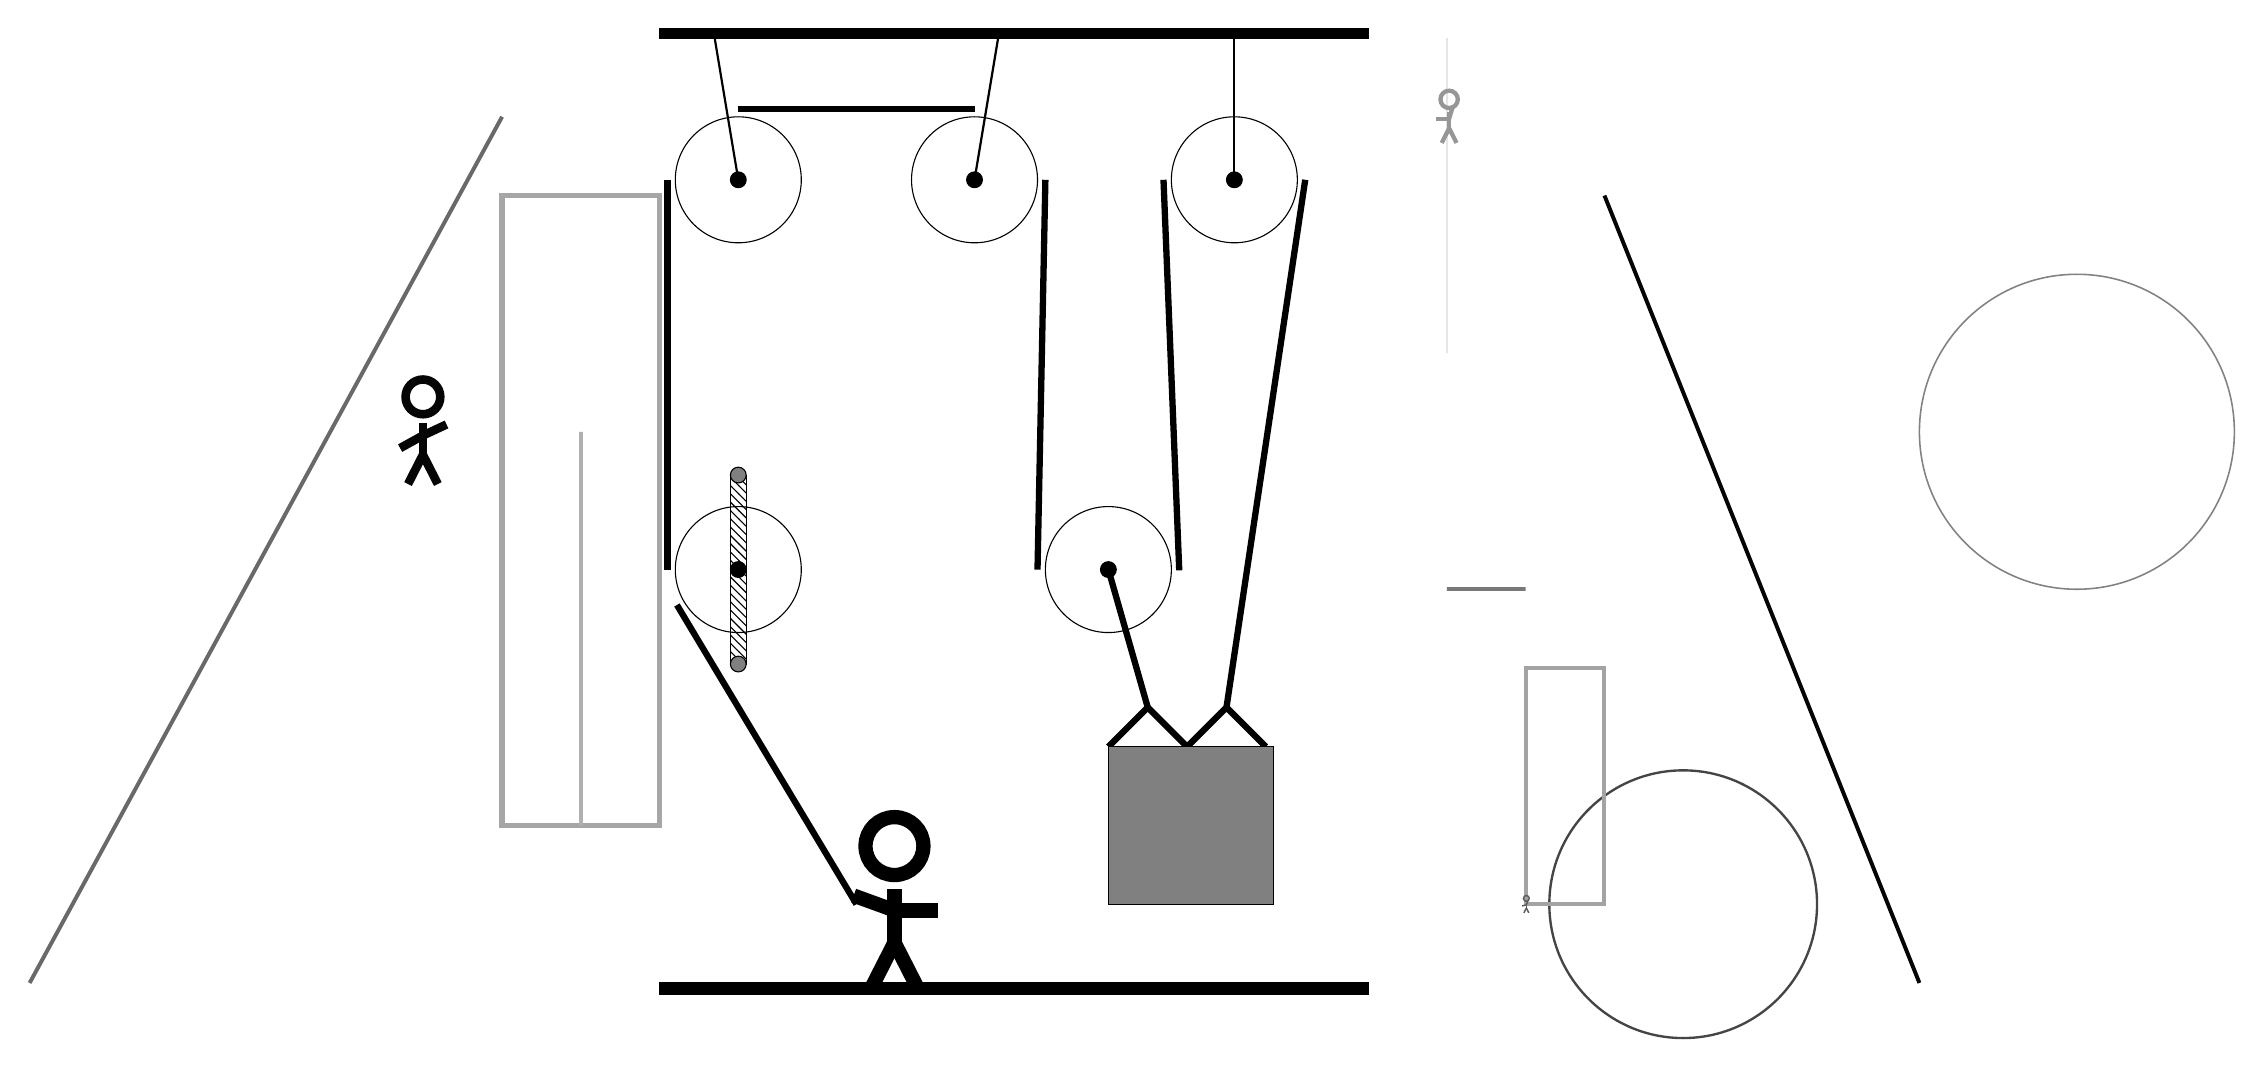
\begin{tikzpicture}
			%%%%% START %%%%%
			
			\draw[fill=black] (-3, 9) rectangle (6, 9.125);
			
			\draw (1, 7.2) circle (0.8);
			\draw[fill=black] (1, 7.2) circle (0.1);
			\draw[thick] (1, 7.2) -- (1.3, 9);
			
			\draw (4.3, 7.2) circle (0.8);
			\draw[fill=black] (4.3, 7.2) circle (0.1);
			\draw[thick] (4.3, 7.2) -- (4.3, 9);
			
			\draw (2.7, 2.25) circle (0.8);
			\draw[fill=black] (2.7, 2.25) circle (0.1);
			
			\draw[line width=0.8mm]  (2.7, 0) -- (3.2, 0.5) -- (3.7, 0) -- (4.2, 0.5) -- (4.7, 0);
			\draw[fill=black!50] (2.7, 0) rectangle (4.8, -2);
			
			\draw (-2, 7.2) circle (0.8);
			\draw[fill=black] (-2, 7.2) circle (0.1);
			\draw[thick] (-2, 7.2) -- (-2.3, 9);
			
			\draw (-2, 2.25) circle (0.8);
			\draw[fill=black] (-2, 2.25) circle (0.1);
			\draw[pattern=north west lines, pattern color=black] (-2.1, 3.45) rectangle (-1.9, 1.05);
			\draw[fill=black!50] (-2, 3.45) circle (0.1);
			\draw[fill=black!50] (-2, 1.05) circle (0.1);
			
			\draw[line width=0.8mm](-0.5, -2) -- (-2.7794, 1.8);
			\centerarc[line width=0.8mm](-2, 2.25)(180:210:0.9);
			\draw[line width=0.8mm](-2.9, 2.25) -- (-2.9, 7.2);
			\centerarc[line width=0.8mm](-2, 7.2)(90:180:0.9);
			
			\draw[line width=0.8mm](-2, 8.1) -- (1, 8.1);
			\centerarc[line width=0.8mm](1, 7.2)(0:90:0.9);
			\draw[line width=0.8mm](1.9, 7.2) -- (1.8, 2.25);
			\centerarc[line width=0.8mm](2.7, 2.25)(180:370:0.9);
			\draw[line width=0.8mm] (3.6, 2.24) -- (3.4, 7.2);
			\centerarc[line width=0.8mm](4.3, 7.2)(0:180:0.9);
			\draw[line width=0.8mm](4.2, 0.5) -- (5.2, 7.2);
			\draw[line width=0.8mm] (3.2, 0.5) -- (2.7, 2.25);
			
			\node at (0, -2) {\Strichmaxerl[10][-20][0]};
			
			\draw[line width=0.3mm, color=black!10] (7, 9) rectangle (7, 5);
			
			\draw[line width=0.7mm, color=black!35] (-5, -1) rectangle (-3, 7);
			\node[line width=0.5mm, color=black!98] at (-6, 4) {\Strichmaxerl[6][29][25]};
			\node[line width=0.2mm, color=black!41] at (7, 8) {\Strichmaxerl[3][0][73]};
			
			\draw[line width=0.5mm, color=black!98](9, 7) -- (13, -3);
			\draw [line width=0.3mm, color=black!73](10, -2) circle (1.7);
			
			\draw[line width=0.5mm, color=black!31] (-4, -1) rectangle (-4, 4);
			
			\draw [line width=0.2mm, color=black!49](15, 4) circle (2.0);
			\draw[line width=0.5mm, color=black!53] (7, 2) rectangle (8, 2);
			\draw[line width=0.5mm, color=black!36] (8, 1) rectangle (9, -2);
			\node[line width=0.6mm, color=black!64] at (8, -2) {\Strichmaxerl[1][15][69]};
			\draw[line width=0.5mm, color=black!59](-5, 8) -- (-11, -3);
			
			\draw[fill=black] (-3, -3) rectangle (6, -3.15);
			
			%%%%% END %%%%%
		\end{tikzpicture}
	\end{figure}	
\end{document}